\documentclass[11pt,a4paper]{article}
\usepackage{float}
\usepackage{verbatim}
\usepackage{subfig}
\usepackage[T1]{fontenc}
\usepackage[utf8]{inputenc}
\usepackage{geometry}
\usepackage{enumitem}
%\geometry{verbose,lmargin=2cm,rmargin=2cm, bmargin=2cm, tmargin=2cm}
\usepackage{wrapfig}
\usepackage{tikz}
\usetikzlibrary{decorations.markings}
\usepackage{calc}
\usepackage{wrapfig}
\usepackage{graphicx}
\usepackage{amssymb}
\usepackage{amsmath}
\usepackage{esint}
\usepackage{multicol}
\usepackage{hyperref}
\usepackage{listings}
\hypersetup{
    colorlinks=true,
    linkcolor=blue,
    filecolor=magenta,
    urlcolor=cyan,
}
\usepackage{listings}
\lstset{ %
  backgroundcolor=\color{white},   % choose the background color; you must add \usepackage{color} or \usepackage{xcolor}; should come as last argument
  basicstyle=\footnotesize,        % the size of the fonts that are used for the code
  breakatwhitespace=false,         % sets if automatic breaks should only happen at whitespace
  breaklines=true,                 % sets automatic line breaking
  captionpos=t,                    % sets the caption-position to bottom
  commentstyle=\color{teal},    % comment style
  deletekeywords={...},            % if you want to delete keywords from the given language
  escapeinside={\%*}{*)},          % if you want to add LaTeX within your code
  extendedchars=true,              % lets you use non-ASCII characters; for 8-bits encodings only, does not work with UTF-8
  frame=single,                    % adds a frame around the code
  keepspaces=true,                 % keeps spaces in text, useful for keeping indentation of code (possibly needs columns=flexible)
  keywordstyle=\color{blue},       % keyword style
 % language=Python,                 % the language of the code
  morekeywords={*,...},           % if you want to add more keywords to the set
  numbers=left,                    % where to put the line-numbers; possible values are (none, left, right)
  numbersep=5pt,                   % how far the line-numbers are from the code
  numberstyle=\tiny\color{black}, % the style that is used for the line-numbers
  rulecolor=\color{black},         % if not set, the frame-color may be changed on line-breaks within not-black text (e.g. comments (green here))
  showspaces=false,                % show spaces everywhere adding particular underscores; it overrides 'showstringspaces'
  showstringspaces=false,          % underline spaces within strings only
  showtabs=false,                  % show tabs within strings adding particular underscores
  stepnumber=1,                    % the step between two line-numbers. If it's 1, each line will be numbered
  tabsize=2,                       % sets default tabsize to 2 spaces
  title=\lstname                   % show the filename of files included with \lstinputlisting; also try caption instead of title
}
\begin{document}



%\preprint{APS/123-QED}

\title{FYS2150 \\ Lab Report: Drag}% Force line breaks with \\

\author{Nicholas Karlsen}
% \email{nichoka@student.matnat.uio.no}

\date{\today}% It is always \today, today,
             %  but any date may be explicitly specified

\maketitle

\begin{abstract}
  A study on the flow of an assortment of spheres in a fluid and the use of image processing to determine the terminal velocity.
\end{abstract}

%\tableofcontents

\begin{multicols*}{2}
\section{\label{sect:intro}Introduction}
  This report contains the description and analysis of data collected in the lab 21.03.2018 concerning the flow of several spherical objects in a large range of different sizes and densities. The balls were immersed in fluid, dropped and filmed. Post-lab, the raw footage was then processed using a Python script in order to quantify the motion of the spheres. This 

\section{\label{sect:theory}Theory}

\section{\label{section:experimental}Experimental Procedure}
  \subsection{Determining framerate of the camera}
    
    

    \begin{figure}[H]
      \center
      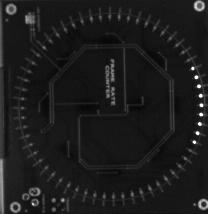
\includegraphics[width=7cm]{scripts/figs/sync_fps.png}
      \caption{Signal used to determine the FPS of the camera}
      \label{fig:FpsSignal}
    \end{figure}
  

  \begin{figure}[H]
    \center
    \subfloat[][Large tube]{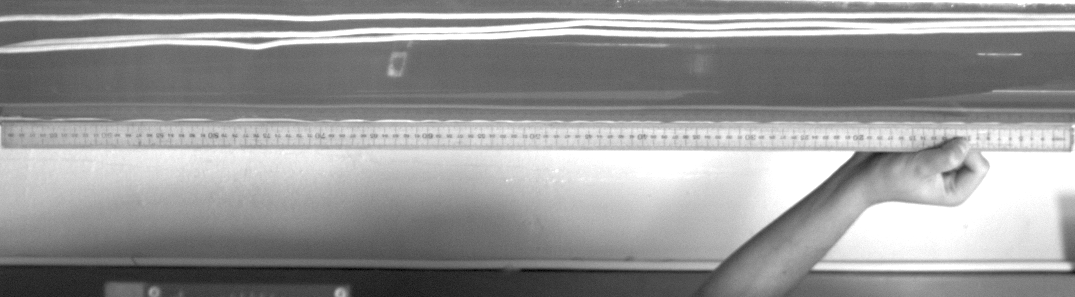
\includegraphics[width=8cm, angle=90]{scripts/figs/bilde_scale1.png}\label{<figure1>}}
    \subfloat[][Small tube]{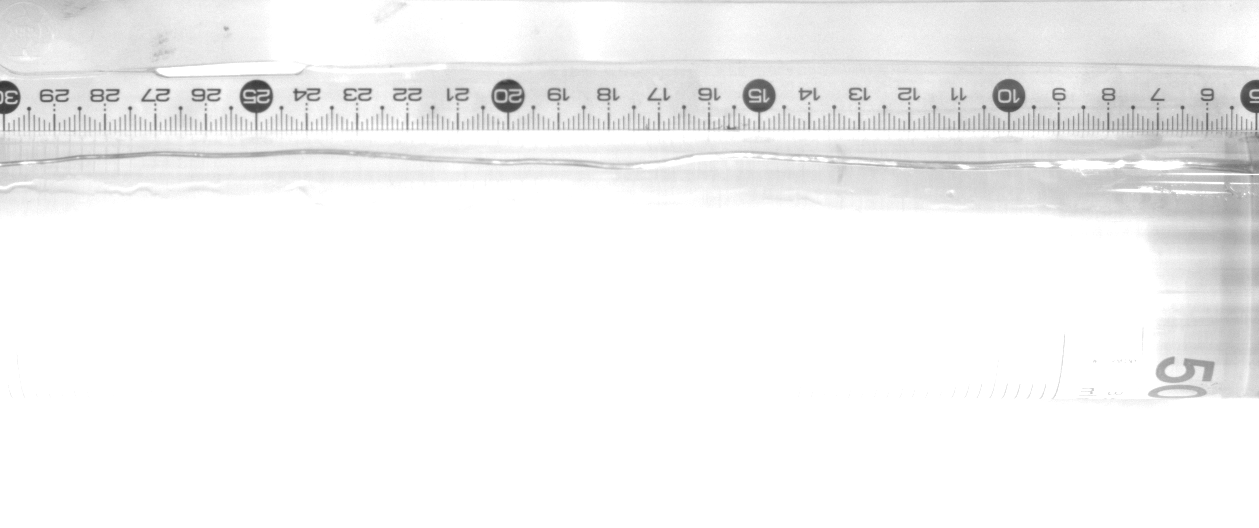
\includegraphics[width=8cm, angle=90]{scripts/figs/bilde_scale2.png}\label{<figure1>}}

    \caption{Cropped images used to find pixel to meter ratio for both of the tubes. (Scaled down in this document)}
    \label{fig:scale1}
  \end{figure}

  \begin{figure}[H]
    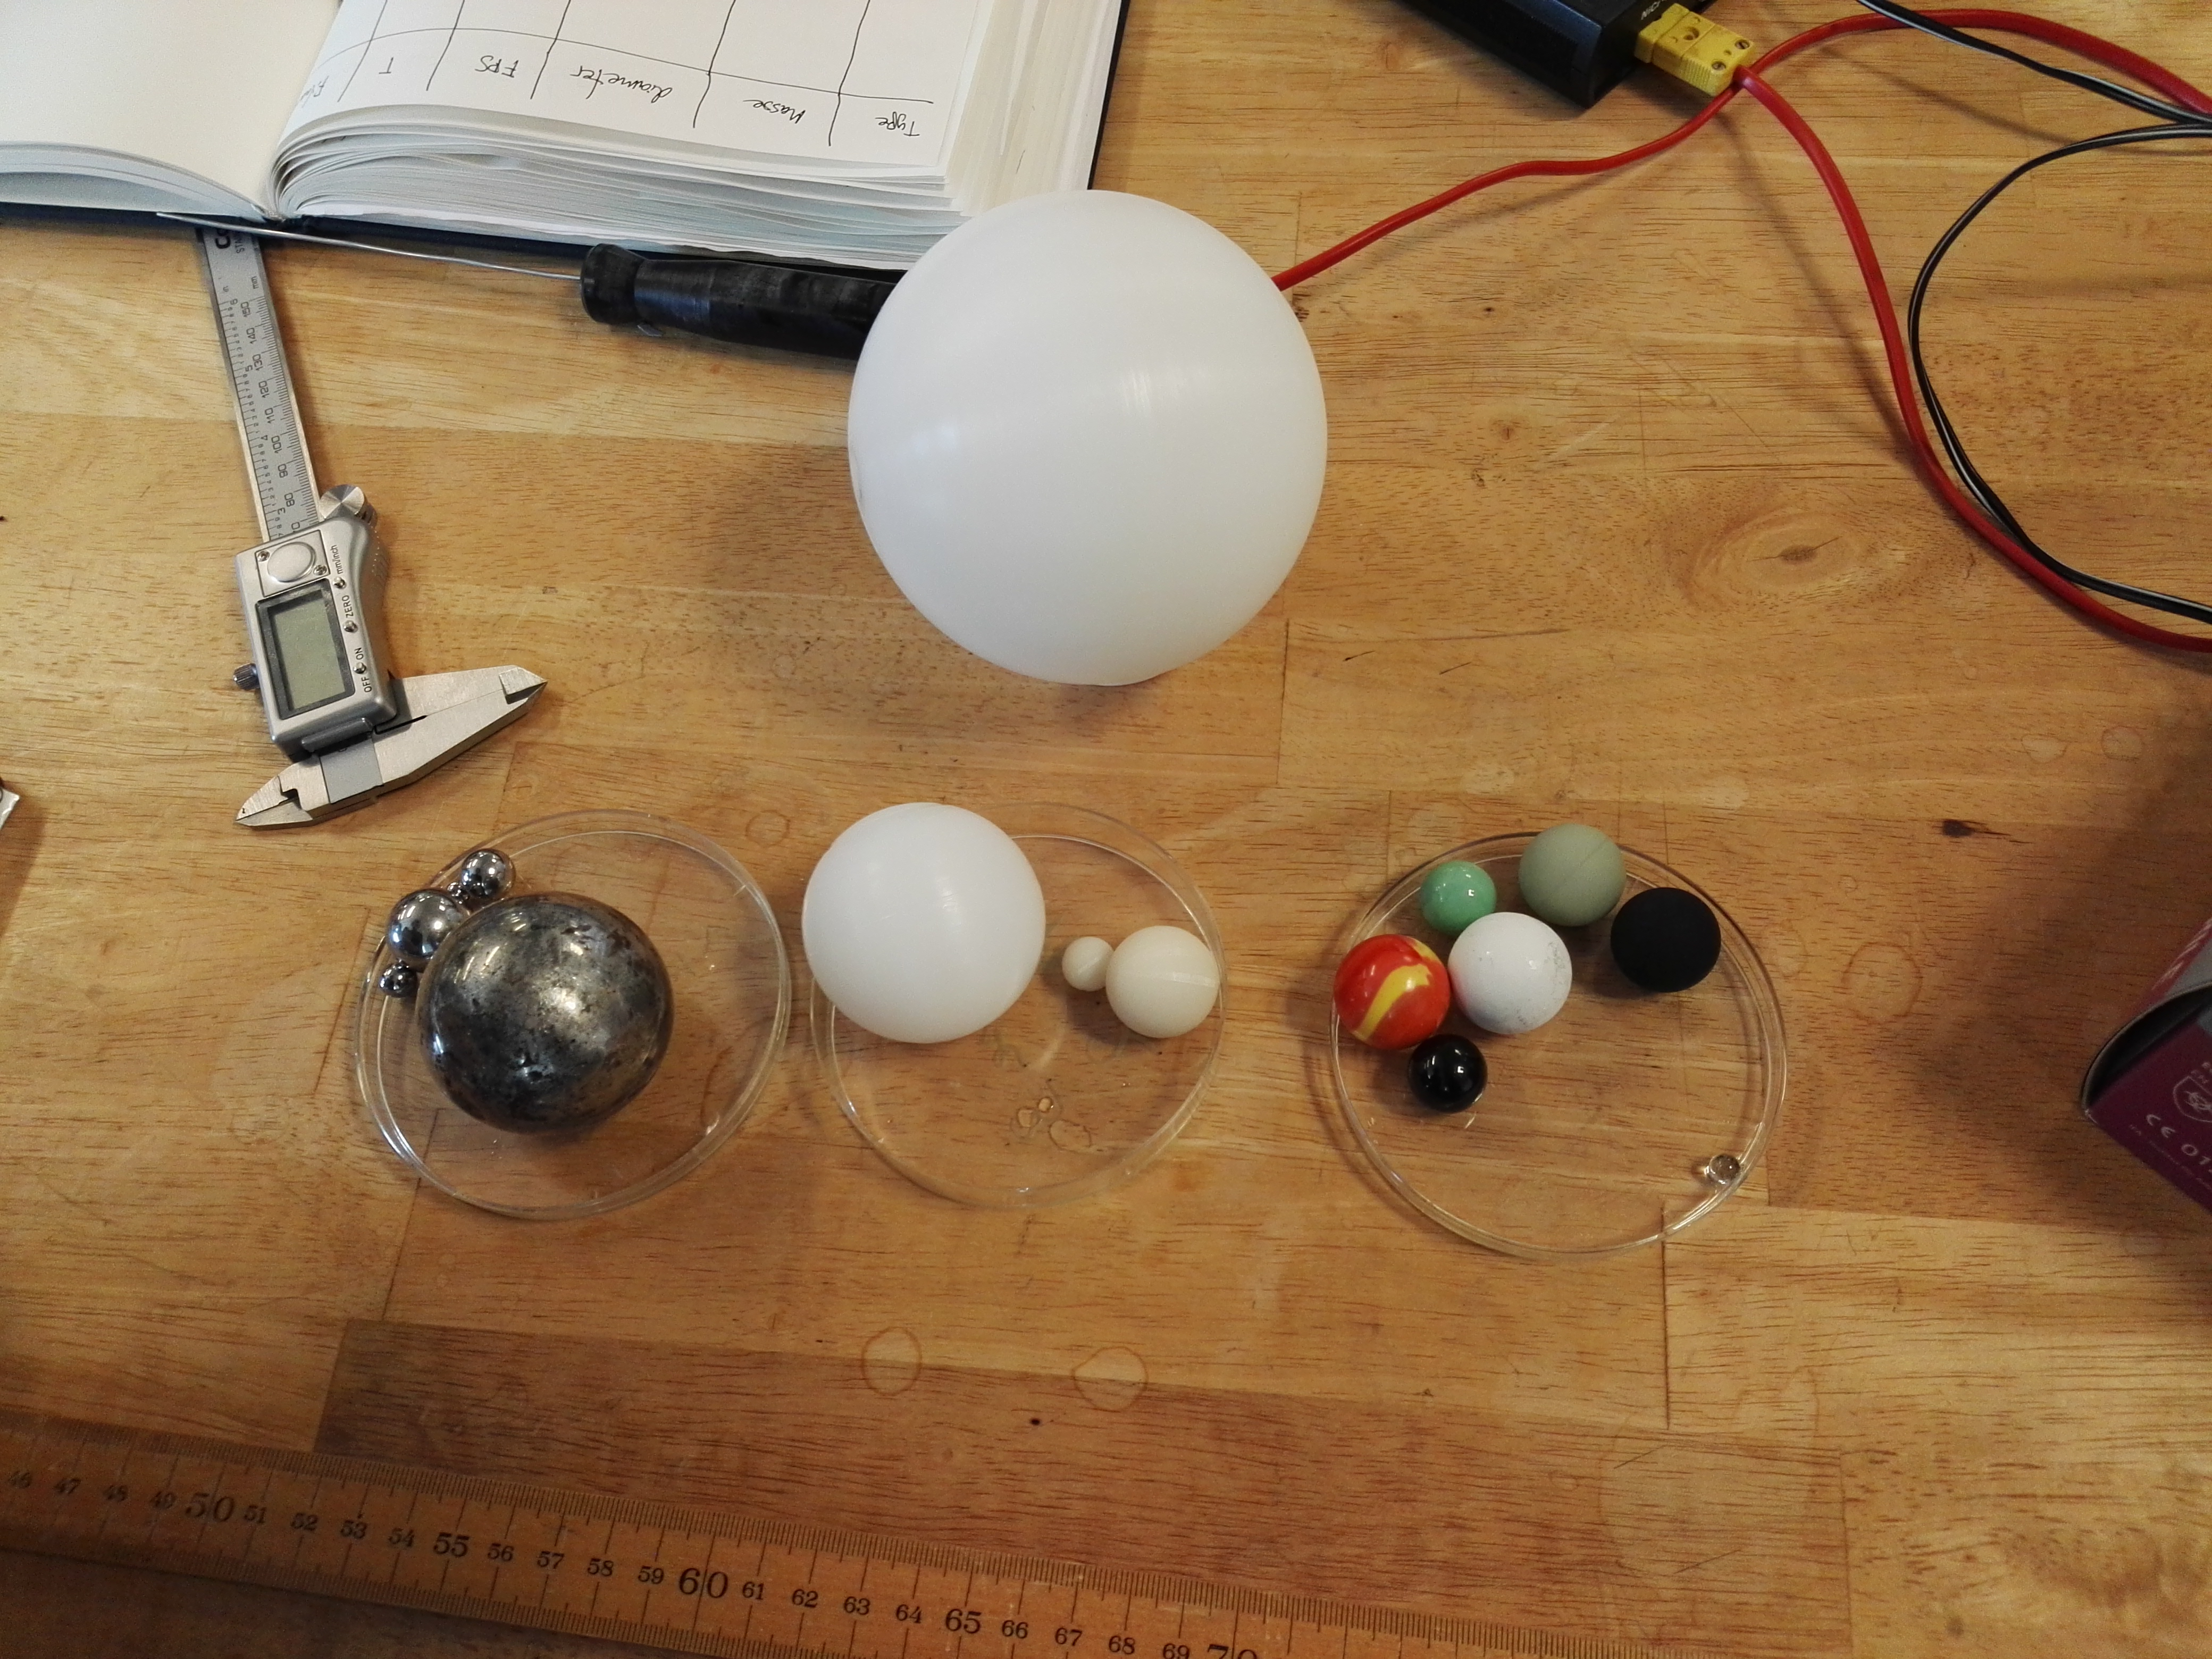
\includegraphics[width=7cm]{scripts/figs/IMG_20180321_131204.jpg}
    \caption{Most of the balls used in the experiment, excluding the ones labeled small 1 and 2.}
  \end{figure}

\section{\label{sect:discuss}Discussion}

\section{\label{sect:results}Results}
  \end{multicols*}

  \begin{table}[H]
    \center
    \begin{tabular}{| l | l | l | l | l | l |}
      \hline
      Type       & Mass[g] & Diameter[mm]   & FPS    & T[C]   & Filena  \\ \hline
      Metal      & 502.76  & 48.98          & 100    & 22.7   & A1.avi  \\ \hline
      Metal      & 28.13   & 19.02          & 100    & 22.8   & A2.avi  \\ \hline 
      Metal      & 6.99    & 11.97          & 100    & 22.6   & A3.avi  \\ \hline
      Metal      & 2.08    & 7.99           & 100    & 22.6   & A4.avi  \\ \hline
      Metal      & 0.68    & 5.48           & 100    & 22.5   & A5.avi  \\ \hline
      Metal      & 0.10    & 2.98           & 100    & 22.6   & A6.avi  \\ \hline
      Plastic    & 488.41  & 99.4           & 100    & 22.5   & B1.avi  \\ \hline
      Plastic    & 61.56   & 50.02          & 100    & 22.5   & B2.avi  \\ \hline
      Plastic    & 7.12    & 23.89          & 100    & 22.6   & B3.avi  \\ \hline
      Plastic    & 0.87    & 12.06          & 100    & 22.6   & B4.avi  \\ \hline
      White      & 29.74   & 25.24          & 100    & 22.6   & C1.avi  \\ \hline
      BigBlack   & 31.42   & 21.08          & 100    & 22.5   & C4.avi  \\ \hline
      SmallBlack & 5.67    & 16.45          & 100    & 22.5   & C5.avi  \\ \hline
      BigGreen   & 31.60   & 21.86          & 100    & 22.4   & C3.avi  \\ \hline
      SmallGreen & 5.60    & 16.38          & 100    & 22.3   & C6.avi  \\ \hline
      BigRed     & 18.44   & 24.01          & 100    & 22.3   & C2.avi  \\ \hline
      Glass      & 0.27    & 5.81           & 100    & 22.3   & C7.avi  \\ \hline
      Small 1    & 4.1e-3  & 1.0            & 100    & 23.7   & D1.avi  \\ \hline
      Small 2    & 12.0e-3 & 1.59           & 100    & 23.7   & D2.avi  \\ \hline   
    \end{tabular}
    \caption{}
  \end{table}
  
  \begin{multicols*}{2}

\section{\label{sect:conclusion}Conclusion}

\end{multicols*}



%%%%%%%%%%%%%%%%%%%%%%%%
%%% END OF MAIN BODY %%%
%%%%%%%%%%%%%%%%%%%%%%%%

\appendix*
\section{Code}
Following

\lstinputlisting[language=python]{scripts/lesVideo_conv.py}
\lstinputlisting{scripts/data/labdata.dat}

\end{document}